% =====================================================================================
%  Paper final — Grupo 06, 1INF02 Aprendizaje de Máquina 2026-2 (PUCP)
%  Compilar con pdflatex (o latexmk -pdf). Requiere la carpeta fig/ y tablas/ junto a este archivo.
%  Las tablas de resultados (tablas/*.tex) se generan con Notebooks/Notebooks Final/generar_tablas.py
%  a partir de los CSV de resultados: no editar a mano; si cambia un resultado, volver a generarlas.
% =====================================================================================
\documentclass[conference]{IEEEtran}
\IEEEoverridecommandlockouts
\usepackage[utf8]{inputenc}
\usepackage[T1]{fontenc}
\usepackage[spanish,es-noshorthands,es-tabla]{babel}
\usepackage{amsmath,amssymb}
\usepackage{graphicx}
\usepackage{booktabs}
\usepackage{array}
\usepackage{multirow}
\newcolumntype{L}[1]{>{\raggedright\arraybackslash}p{#1}}
\usepackage{url}
\usepackage[hidelinks]{hyperref}
\DeclareUnicodeCharacter{2212}{\ensuremath{-}}
\DeclareUnicodeCharacter{2264}{\ensuremath{\leq}}
\DeclareUnicodeCharacter{2265}{\ensuremath{\geq}}
\DeclareUnicodeCharacter{2248}{\ensuremath{\approx}}
\DeclareUnicodeCharacter{2192}{\ensuremath{\rightarrow}}
\DeclareUnicodeCharacter{03BA}{\ensuremath{\kappa}}
% Todo el documento en Times: \texttt y \url usan Times en lugar de Courier
\renewcommand{\ttdefault}{ptm}
\urlstyle{rm}
% Tablas: datos a 7 pt. \ajustar NUNCA agranda; solo reduce si la tabla excede la columna (y lo avisa en main.log)
\newcommand{\tablesize}{\fontsize{7}{8.4}\selectfont}
\newsavebox{\tabbox}
\newcommand{\ajustar}[1]{%
  \sbox{\tabbox}{#1}%
  \ifdim\wd\tabbox>\columnwidth
    \typeout{AVISO-TABLA: tabla mas ancha que la columna (\the\wd\tabbox\space > \the\columnwidth); se reduce}%
    \resizebox{\columnwidth}{!}{\usebox{\tabbox}}%
  \else
    \usebox{\tabbox}%
  \fi}
\newcommand{\tabla}[1]{\tablesize\setlength{\tabcolsep}{2pt}\ajustar{\input{tablas/#1}}}

\makeatletter
\newcommand{\linebreakand}{%
  \end{@IEEEauthorhalign}
  \hfill\mbox{}\par
  \mbox{}\hfill\begin{@IEEEauthorhalign}
}
\makeatother

\begin{document}

\title{Predicción de la impuntualidad en una ruta de transporte público urbano de Cusco mediante aprendizaje automático: contexto del itinerario frente a información en ruta}

\author{
\IEEEauthorblockN{Jafeth Manases Cuyo Alata}
\IEEEauthorblockA{Facultad de Ciencias e Ingeniería\\
Pontificia Universidad Católica del Perú\\
Lima, Perú\\
jafeth.cuyo@pucp.edu.pe}
\and
\IEEEauthorblockN{Raul Esteban Herrera Guerrero}
\IEEEauthorblockA{Facultad de Ciencias e Ingeniería\\
Pontificia Universidad Católica del Perú\\
Lima, Perú\\
rherrerag@pucp.edu.pe}
\and
\IEEEauthorblockN{Matias Esteban Marrufo Zapata}
\IEEEauthorblockA{Facultad de Ciencias e Ingeniería\\
Pontificia Universidad Católica del Perú\\
Lima, Perú\\
a20230314@pucp.edu.pe}
\linebreakand
\IEEEauthorblockN{Joel Cesar Galindo Nuñez}
\IEEEauthorblockA{Facultad de Ciencias e Ingeniería\\
Pontificia Universidad Católica del Perú\\
Lima, Perú\\
a20200622@pucp.edu.pe}
}

\maketitle

\begin{abstract}
La impuntualidad del transporte público urbano reduce la confiabilidad del servicio y prolonga la espera de los usuarios. Este trabajo predice el retraso con que los buses de una ruta urbana de Cusco terminan su vuelta, a partir de los registros de un sistema de transporte inteligente: 4\,707 vueltas con horas programadas y reales de paso por 18 puntos de control y 1\,630\,431 registros GPS de 45 vehículos, de enero de 2025. Se plantean una tarea de regresión (retraso final en minutos) y una de clasificación en tres clases (adelantado, puntual y retrasado), en cuatro momentos de la vuelta: antes de la salida y tras observar 4, 8 y 12 puntos de control. Se compararon Regresión Ridge/Logística, Random Forest y XGBoost frente a líneas base de persistencia y promedio histórico, con validación cruzada temporal de ventana expansiva, una búsqueda en malla de 4\,165 configuraciones y un conjunto de prueba de 758 vueltas usado una sola vez. Antes de la salida, XGBoost alcanza un MAE de 2,65~min frente a 4,35~min del promedio histórico ($-39$\,\%), un F1-macro de 0,740 frente a 0,248 de la clase mayoritaria y una exactitud de 0,78 con kappa de 0,60 ($p < 0{,}002$ en las 26 comparaciones con las líneas base). La información en ruta solo reduce el error de forma significativa al pasar de 8 a 12 puntos de control (2,64 $\rightarrow$ 2,37~min), y los agregados GPS no aportan mejora. Las variables del estado del día en curso, evaluadas con una regla de aceptación fijada de antemano, tampoco mejoran la validación. La hora de salida y el día de la semana dominan la importancia por permutación y las explicaciones SHAP: los sábados las vueltas terminan, en promedio, 10,4~min tarde. El retraso es en gran medida sistemático, lo que sugiere que recalibrar el itinerario por franja horaria y día puede ser tan útil como el control en tiempo real.
\end{abstract}

\begin{IEEEkeywords}
transporte público, puntualidad, cumplimiento del itinerario, aprendizaje automático, Random Forest, XGBoost, SHAP, datos AVL/GPS, Cusco.
\end{IEEEkeywords}

% =====================================================================================
\section{Introducción}

El transporte público por bus es el principal modo de movilidad en muchas ciudades latinoamericanas, y su atractivo depende en buena medida de la confiabilidad del servicio. Los sistemas de transporte inteligente (STI) equipados con localización automática de vehículos (AVL, por sus siglas en inglés) y GPS registran de forma continua la posición de cada unidad y su paso por puntos de control, lo que permite medir con precisión el cumplimiento del itinerario y abordar su predicción con técnicas de aprendizaje automático~\cite{alexandre2023,singh2022}.

En una ruta urbana, el retraso se define como la diferencia entre la hora real y la hora programada de paso; un valor negativo indica que el bus va adelantado~\cite{lin1999}. Ambos sentidos son fallas de servicio: el retraso prolonga la espera, y el adelanto hace que el usuario que llega a tiempo pierda el bus. El problema es relevante incluso en grandes sistemas; con datos de Nueva York se reporta un retraso promedio cercano a ocho minutos entre la llegada programada y la real~\cite{rashvand2024}.

Este trabajo estudia una ruta de transporte público de Cusco que conecta el extremo este de la ciudad con el centro histórico a través de la Av.~de la Cultura. La observación de campo de los autores sugiere varias causas de desviación: los buses esperan en paraderos concurridos para captar pasajeros, hay congestión en zonas comerciales como el entorno del mercado San Pedro y en los accesos a la Av.~de la Cultura, y se suman pendientes pronunciadas y una regulación limitada de la operación. Tras la depuración, el 27,7\,\% de las vueltas termina con más de 5~min de retraso y el 17,0\,\% con más de 1~min de adelanto.

La pregunta que guía el estudio es si es posible anticipar el retraso con que un bus terminará su vuelta y en qué momento de la vuelta la predicción resulta útil para la gestión de la flota. Las contribuciones son:
\begin{itemize}
\item Un procedimiento reproducible de integración y depuración de los dos conjuntos de datos del STI, que documenta inconsistencias de los registros y verifica numéricamente la semántica de sus columnas.
\item Una formulación que contrasta la predicción antes de la salida, basada solo en el contexto del itinerario, con la predicción actualizada tras 4, 8 y 12 puntos de control, con y sin variables GPS.
\item La comparación de tres familias de modelos frente a dos líneas base, bajo validación temporal, con pruebas estadísticas pareadas y con un protocolo de mejoras cuyas reglas de aceptación se fijaron antes de ver los resultados.
\item Evidencia, por importancia de variables y explicaciones SHAP, de que el retraso es mayormente sistemático (hora de salida y día de la semana), con implicancias para la recalibración del itinerario.
\end{itemize}

El documento se organiza así: la Sección~\ref{sec:obj} plantea los objetivos e hipótesis; la \ref{sec:rel} revisa los trabajos relacionados; la \ref{sec:datos} describe el dataset y el análisis exploratorio; la \ref{sec:met} detalla la metodología; la \ref{sec:res} presenta los resultados; la \ref{sec:disc} los discute; la \ref{sec:lim} expone las limitaciones, y la \ref{sec:conc} concluye.

% =====================================================================================
\section{Objetivos e hipótesis}\label{sec:obj}

\subsection{Objetivo general}
Desarrollar y evaluar modelos de aprendizaje automático que predigan el retraso con que un bus de transporte público de Cusco finaliza su vuelta, comparando la predicción antes de la salida con la actualizada durante el recorrido, para identificar los factores que determinan la impuntualidad y apoyar la gestión del itinerario.

\subsection{Objetivos específicos}
\begin{itemize}
\item[OE1.] Integrar y depurar los conjuntos Times y Monitoring: transformar las listas por punto de control, tratar faltantes y valores atípicos, cruzar ambos conjuntos y ubicar los puntos de control.
\item[OE2.] Caracterizar los patrones de retraso por franja horaria, día de la semana y tramo de la ruta.
\item[OE3.] Implementar y comparar modelos de regresión y clasificación frente a líneas base de persistencia y promedio histórico.
\item[OE4.] Cuantificar el aporte de los retrasos observados en ruta ($k = 0, 4, 8, 12$ puntos de control) y de las variables derivadas del GPS frente al contexto del itinerario.
\item[OE5.] Identificar los factores más influyentes mediante importancia de variables y explicaciones SHAP, y discutir sus implicancias para el itinerario.
\end{itemize}

\subsection{Hipótesis}
\textbf{H1.} Los modelos de aprendizaje automático obtienen un error menor que las líneas base de persistencia y promedio histórico. \textbf{H2.} El error de predicción disminuye a medida que aumenta el número $k$ de puntos de control observados. \textbf{H3.} Las variables derivadas del GPS reducen el error respecto de usar solo los registros de puntos de control.

% =====================================================================================
\section{Trabajos relacionados}\label{sec:rel}

\subsection{Predicción de llegada y retraso con datos AVL/GPS}
Lin y Zeng~\cite{lin1999} desarrollaron cuatro algoritmos de estimación de la llegada del bus que usan información creciente y concluyeron que el tiempo de permanencia en paradas de control horario es el factor más relevante, hallazgo vinculado con las esperas en paraderos concurridos observadas en Cusco. Jeong y Rilett~\cite{jeong2005} propusieron modelos de predicción de llegada con datos AVL que consideran el cumplimiento del horario y los tiempos de permanencia en paradas. Liu et~al.~\cite{liu2020} compararon modelos de retraso, $k$ vecinos más cercanos, regresión kernel, modelo aditivo y LSTM. Rashvand et~al.~\cite{rashvand2024} emplearon una red neuronal densa sobre datos de Nueva York y superaron a SVR.

\subsection{Ensambles de árboles para la puntualidad}
Martyanov et~al.~\cite{martyanov2026} predicen el retraso por parada con datos AVL; Random Forest, XGBoost y CatBoost alcanzaron una precisión comparable (RMSE $\approx$ 5,4~min; MAE $\approx$ 3,6~min; $R^2 \approx$ 0,44) con validación cruzada temporal anidada. Meyer-Hollatz et~al.~\cite{meyer2023} mostraron con XGBoost que añadir clima y feriados mejoró el MAE en 17,33\,\% respecto de usar solo AVL y características del horario, un diseño de ablación análogo al de H3. En la tesis de Taparia~\cite{taparia2020}, Gradient Boosting superó al promedio histórico y a la regresión lineal. Cao et~al.~\cite{cao2017} clasificaron la puntualidad en tres clases con Random Forest, con umbrales de 80~s de adelanto y 320~s de retraso.

\subsection{Predicción con anticipación y revisiones}
Sun et~al.~\cite{sun2021} predijeron con regresión logística la probabilidad de apelotonamiento usando registros GPS de al menos $k$ paradas aguas arriba, y Yu et~al.~\cite{yu2016} lo detectaron con máquinas de vectores de soporte. Estos trabajos inspiran el análisis por número de puntos de control observados y el énfasis en la sensibilidad y la especificidad de la clase de interés. Alexandre et~al.~\cite{alexandre2023} y Singh y Kumar~\cite{singh2022} ofrecen revisiones del área.

\subsection{Síntesis y brecha}
La Tabla~\ref{tab:antecedentes} resume los antecedentes más cercanos. La mayoría predice la llegada o el retraso en la siguiente parada; pocos contrastan cuánto se puede anticipar antes de la salida frente a lo que añade la información en ruta. No se encontraron estudios aplicados a ciudades peruanas.

\begin{table}[!t]
\centering
\caption{Antecedentes más cercanos a la propuesta}\label{tab:antecedentes}
\tablesize\setlength{\tabcolsep}{2pt}
\begin{tabular}{@{}L{0.06\columnwidth}L{0.20\columnwidth}L{0.18\columnwidth}L{0.27\columnwidth}L{0.20\columnwidth}@{}}
\toprule
Ref. & Datos & Tarea & Modelos & Evaluación \\
\midrule
\cite{lin1999} & GPS, Blacksburg (EE.\,UU.) & Llegada a parada & 4 algoritmos, info. creciente & Precisión, robustez \\
\cite{liu2020} & GPS de buses (gran escala) & Tiempo de llegada & Retraso, $k$-NN, kernel, LSTM & RMSE comparativo \\
\cite{martyanov2026} & AVL + horario & Retraso por parada & RF, XGBoost, CatBoost & CV temporal anidada \\
\cite{meyer2023} & AVL (3 años) + clima & Retraso de salida & 4 modelos; mejor XGBoost & MAE; ablación \\
\cite{taparia2020} & AVL/GPS archivados & Llegada y viaje & Prom. hist., LR, GB, LSTM & Conjunto de prueba \\
\cite{cao2017} & Buses + GTFS & Puntualidad (3 clases) & Random Forest & CV de 10 pliegues \\
\cite{sun2021} & GPS, Kioto & Apelotonamiento & Logística, SVM & ROC \\
\bottomrule
\end{tabular}
\end{table}

% =====================================================================================
\section{Descripción del dataset}\label{sec:datos}

\subsection{Origen}
Los datos provienen de un STI del transporte público de Cusco y fueron proporcionados en dos archivos: \texttt{Times.csv} (registros de paso por puntos de control) y \texttt{Monitoring.csv} (registros georreferenciados). Ambos comparten el identificador del vehículo, la fecha y el número de vuelta, que se usan como llave de cruce.

\subsection{Registros de puntos de control (Times.csv)}
Contiene 4\,707 vueltas de 45 vehículos en 27 días consecutivos (06/01/2025 al 01/02/2025). Cada fila es una vuelta completa con 18 puntos de control (PC), y tres de sus columnas son listas de 18 valores (Tabla~\ref{tab:vars}). El README describe \texttt{difference\_time} como la diferencia entre \texttt{end\_time} y \texttt{start\_time}; la verificación numérica muestra que \texttt{start\_time} contiene las horas programadas, \texttt{end\_time} las horas reales, y que la desviación corresponde a~\eqref{eq:dev}, con coincidencia en el 100\,\% de los 76\,980 valores válidos:
\begin{equation}\label{eq:dev}
d_{i,j} = \operatorname{trunc}\left[\left(t^{\text{real}}_{i,j} - t^{\text{prog}}_{i,j}\right)/60\right]
\end{equation}
donde $d_{i,j}$ es la desviación en minutos de la vuelta $i$ en el PC $j$, truncada hacia cero. Un valor negativo indica adelanto y uno positivo, retraso. % TODO: actualizar si los docentes confirman la semántica de difference_time.
Esta interpretación está pendiente de confirmación por los docentes.

\begin{table}[!t]
\centering
\caption{Variables de Times.csv (semántica verificada)}\label{tab:vars}
\tablesize
\begin{tabular}{@{}lp{5.6cm}@{}}
\toprule
Columna & Contenido \\
\midrule
\texttt{id} & Identificador del registro (vuelta) \\
\texttt{lap} & Número de vuelta del vehículo en el día (1 a 8) \\
\texttt{date}, \texttt{time} & Fecha y hora programada de salida (igual al primer valor de \texttt{start\_time}) \\
\texttt{start\_time} & Lista de 18 horas programadas de paso (PC1\ldots PC18) \\
\texttt{end\_time} & Lista de 18 horas reales de paso \\
\texttt{difference\_time} & Lista de 18 desviaciones en minutos según~\eqref{eq:dev}; ``-'' indica faltante \\
\texttt{vehicle\_id\_id} & Identificador del vehículo (45 unidades) \\
\bottomrule
\end{tabular}
\end{table}

\subsection{Registros georreferenciados (Monitoring.csv)}
Contiene 1\,630\,431 registros de 9 variables (fecha, hora, vuelta, latitud, longitud, velocidad, rumbo y vehículo) de los mismos 45 vehículos, entre el 01/01/2025 y el 01/02/2025, sin valores nulos. El intervalo mediano entre registros consecutivos de un vehículo es de 25~s, pero depende de la velocidad: 75~s con el bus detenido ($\leq$ 2~km/h), 25~s entre 20 y 40~km/h y 12~s por encima de 40~km/h. Por ello, el tiempo detenido se mide como duración y no como conteo de registros. El cruce con \texttt{Times.csv} cubre el 99,9\,\% de las vueltas, con unos 300 registros GPS por vuelta; los registros del 01 al 05 de enero y los de vuelta~0 no tienen contraparte.

\subsection{Ruta y puntos de control}
Los PC se ubicaron tomando, para cada vuelta, el registro GPS más cercano en el tiempo ($\pm$30~s) a la hora real de paso, y calculando la mediana de las coordenadas sobre una muestra de 1\,500 vueltas; la desviación mediana respecto de esa ubicación es de 25 a 50~m según el PC. La ruta es de ida y vuelta (Fig.~\ref{fig:ruta}): parte del extremo este (PC1), llega al punto más occidental (PC10) y retorna hasta PC18, ubicado a 894~m de PC1. El orden de los PC es siempre el mismo: en más del 99,6\,\% de las vueltas la posición GPS al pasar por PC1, PC10 y PC18 está a menos de 300~m de su ubicación de referencia. Por ello, cada vuelta tiene una sola variable objetivo: la desviación en PC18. La Tabla~\ref{tab:pc} describe los PC.

\begin{figure}[!t]
\centering
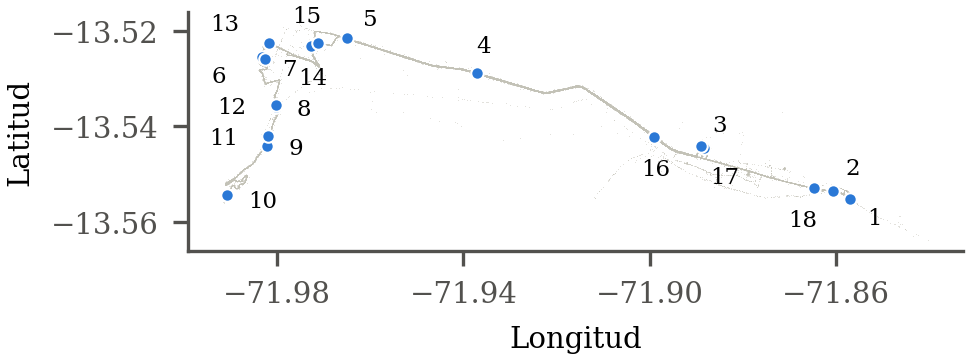
\includegraphics[width=\columnwidth]{fig/paper_fig1_ruta.png}
\caption{Ruta estudiada y ubicación de los 18 puntos de control estimada a partir del GPS. En gris, una muestra de 60\,000 registros GPS.}\label{fig:ruta}
\end{figure}

\begin{table}[!t]
\centering
\caption{Puntos de control de la ruta}\label{tab:pc}
\tablesize\setlength{\tabcolsep}{2.5pt}
\begin{tabular}{@{}clcl@{}}
\toprule
PC & Lat., Lon. & $t$ (min) & Descripción \\
\midrule
1 & $-$13,5552; $-$71,8568 & 0 & Inicio de la vuelta (extremo este) \\
2 & $-$13,5535; $-$71,8606 & 2 & Punto concurrido \\
3 & $-$13,5445; $-$71,8883 & 13 & Punto concurrido \\
4 & $-$13,5288; $-$71,9372 & 30 & Av.~de la Cultura \\
5 & $-$13,5216; $-$71,9651 & 43 & Av.~de la Cultura, cerca del centro \\
6 & $-$13,5256; $-$71,9833 & 61 & Punto concurrido \\
7 & $-$13,5259; $-$71,9827 & 62 & Punto concurrido \\
8 & $-$13,5359; $-$71,9804 & 68 & Punto concurrido \\
9 & $-$13,5441; $-$71,9821 & 74 & Punto concurrido \\
10 & $-$13,5543; $-$71,9908 & 84 & Punto más occidental (retorno) \\
11 & $-$13,5419; $-$71,9821 & 93 & Punto concurrido \\
12 & $-$13,5355; $-$71,9804 & 97 & Punto concurrido \\
13 & $-$13,5226; $-$71,9818 & 109 & Inmediaciones del mercado San Pedro \\
14 & $-$13,5233; $-$71,9728 & 115 & Av.~Tullumayo, acceso a la Av.~de la Cultura \\
15 & $-$13,5226; $-$71,9714 & 119 & Punto concurrido \\
16 & $-$13,5423; $-$71,8991 & 147 & Av.~de la Cultura \\
17 & $-$13,5441; $-$71,8888 & 150 & Punto concurrido \\
18 & $-$13,5529; $-$71,8648 & 161 & Fin de la vuelta (extremo este) \\
\bottomrule
\end{tabular}

\vspace{2pt}\raggedright\scriptsize $t$: minutos desde la salida en el horario programado de 161~min, el más frecuente. Descripciones según la observación de campo de los autores.
\end{table}

\subsection{Calidad de los datos}
La Tabla~\ref{tab:calidad} resume los problemas detectados y su tratamiento. Tras la depuración quedan 4\,559 vueltas, de las cuales 4\,004 tienen retraso final válido y solo cuatro horarios programados distintos (147, 161, 168 y 170~min).

\begin{table}[!t]
\centering
\caption{Problemas de calidad y tratamiento}\label{tab:calidad}
\tablesize\setlength{\tabcolsep}{2.5pt}
\begin{tabular}{@{}p{2.9cm}p{2.3cm}p{2.6cm}@{}}
\toprule
Problema & Magnitud & Tratamiento \\
\midrule
Desviación ``-'' (hora real corrupta) & 7\,746 de 84\,726 PC (9,14\,\%) & Faltante; la hora real no se usa \\
Desviación $|d| > 60$~min & 156 PC & Faltante (atípico) \\
Horario programado no monótono & 148 vueltas (3,1\,\%) & Excluir la vuelta \\
PC18 sin valor válido & 555 vueltas & Excluir del modelado \\
Faltantes en PC1\ldots PC17 de vueltas válidas & 1\,354 valores en 935 vueltas & Imputación o manejo nativo (V-C) \\
GPS duplicado (vehículo, fecha, hora) & 6\,783 registros & Eliminar \\
Velocidad GPS alta & 10 registros $>$ 90~km/h (máx.~107) & Se conservan: efecto despreciable \\
\bottomrule
\end{tabular}
\end{table}

\subsection{Análisis exploratorio}
El retraso final en PC18 tiene media de 2,72~min, mediana de 2~min y desviación estándar de 8,22~min. Con los umbrales de la Sección~\ref{sec:form}, las clases adelantado, puntual y retrasado representan el 17,0\,\%, 55,3\,\% y 27,7\,\% de las vueltas.

\textbf{Horario y hora de salida.} El retraso depende fuertemente del horario programado (Tabla~\ref{tab:horario}) y de la hora de salida (Fig.~\ref{fig:horadia}a): $-$20,0~min de media a las 4~h y +11,3~min a las 17~h. Las vueltas del horario de 147~min (salida mediana 5:50) terminan en promedio 5,1~min adelantadas, mientras que en el horario de 170~min el 53,7\,\% termina con más de 5~min de retraso, pese a que ese horario asigna más tiempo. El patrón es coherente con la demanda: en la madrugada hay pocos pasajeros y no hay motivo para esperar en los paraderos; al mediodía y por la tarde las esperas se prolongan.

\begin{table}[!t]
\centering
\caption{Retraso final según el horario programado}\label{tab:horario}
\tablesize\setlength{\tabcolsep}{2.5pt}
\begin{tabular}{@{}lccccc@{}}
\toprule
Duración prog. & Vueltas & Salida (med.) & Media (min) & \% retr.\,$>$\,5 & \% adel.\,$>$\,1 \\
\midrule
147 min & 642 & 5:50 & $-$5,09 & 12,3 & 52,8 \\
161 min & 2\,700 & 11:02 & +3,91 & 26,0 & 10,3 \\
168 min & 178 & 17:45 & +3,89 & 39,3 & 13,5 \\
170 min & 484 & 17:37 & +6,00 & 53,7 & 8,1 \\
\bottomrule
\end{tabular}
\end{table}

\textbf{Día de la semana.} El sábado destaca con un retraso medio de +10,4~min, frente a +0,7 a +2,1~min de lunes a viernes y +3,8~min el domingo (Fig.~\ref{fig:horadia}b). Los cuatro sábados del periodo varían entre sí: +7,8 (11/01), +9,0 (18/01), +13,3 (25/01) y +12,1~min (01/02).

\begin{figure}[!t]
\centering
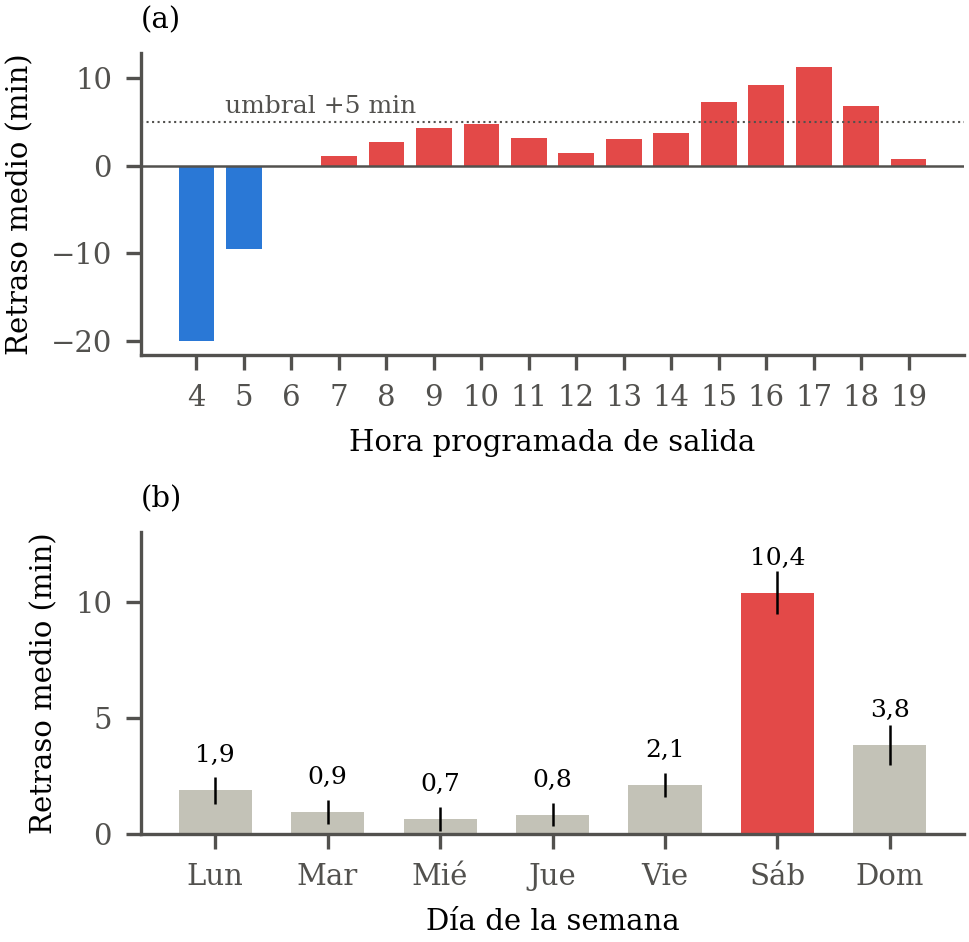
\includegraphics[width=\columnwidth]{fig/paper_fig2_hora_dia.png}
\caption{Retraso medio en PC18 (a) según la hora programada de salida (horas con al menos 30 vueltas; rojo: retraso, azul: adelanto) y (b) según el día de la semana (barras de error: intervalo de confianza del 95\,\%).}\label{fig:horadia}
\end{figure}

\textbf{Tramos.} La Fig.~\ref{fig:tramos} muestra dónde se genera el retraso. El tramo PC13--PC14, del mercado San Pedro a la Av.~Tullumayo, añade en promedio 2,79~min, y el tramo PC5--PC6, junto al centro histórico, 1,17~min. En cambio, el tramo PC14--PC15 recupera 1,96~min pese a que ambos PC distan unos 175~m, lo que sugiere un punto de regulación o espera. El tramo PC15--PC16, que recorre la Av.~de la Cultura, es el más variable (desviación estándar de 3,34~min).

\begin{figure}[!t]
\centering
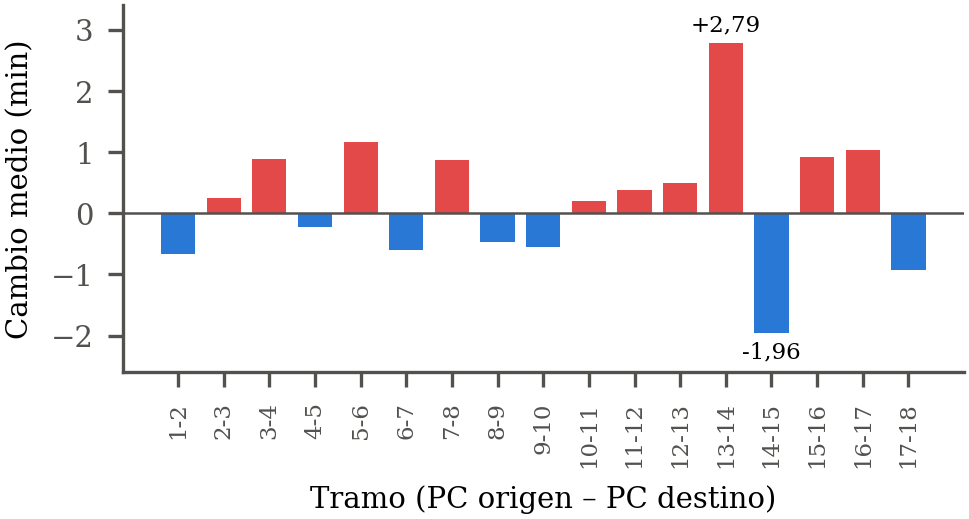
\includegraphics[width=\columnwidth]{fig/paper_fig3_tramos.png}
\caption{Cambio medio de la desviación en cada tramo entre puntos de control consecutivos. Valores positivos: el tramo genera retraso; negativos: el bus recupera tiempo.}\label{fig:tramos}
\end{figure}

\textbf{Información de cada PC.} La correlación entre la desviación en el PC $k$ y la final es casi nula en PC1--PC3 ($-$0,08 a 0,03), sube a 0,40 en PC4, 0,73 en PC8 y 0,76 en PC12, y salta a 0,85 en PC13 y 0,97 en PC16 (Fig.~\ref{fig:corr}). Esto anticipa que la información en ruta aporte poco en la primera mitad de la vuelta y motiva los escenarios $k = 4$, 8 y 12.

\begin{figure}[!t]
\centering
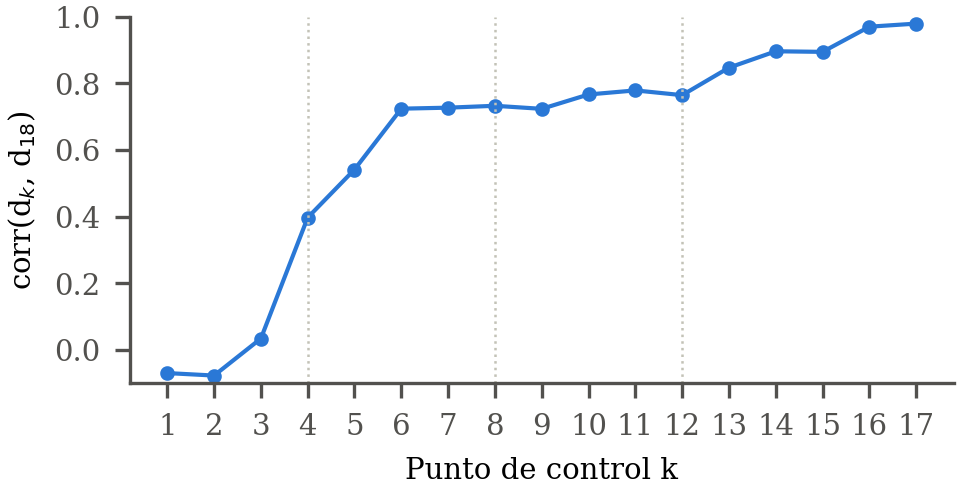
\includegraphics[width=\columnwidth]{fig/paper_fig4_corr_k.png}
\caption{Correlación entre la desviación en el PC $k$ y la desviación final en PC18. Las líneas punteadas marcan los escenarios $k = 4$, 8 y 12.}\label{fig:corr}
\end{figure}

% =====================================================================================
\section{Metodología}\label{sec:met}

\subsection{Formulación del problema}\label{sec:form}
Para la vuelta $i$, la variable objetivo de regresión es $y_i = d_{i,18}$. La predicción en el momento $k$, tras observar $k$ puntos de control, es:
\begin{equation}
\hat{y}^{(k)}_i = f_k\left(\mathbf{x}^{(k)}_i\right), \qquad k \in \{0, 4, 8, 12\}
\end{equation}
donde $\mathbf{x}^{(k)}_i$ reúne las variables disponibles hasta el paso real por el PC $k$; el caso $k = 0$ corresponde a la predicción antes de la salida. Para la clasificación, cada vuelta se asigna a una de tres clases:
\begin{equation}
c_i = \begin{cases} \text{adelantado}, & y_i < -1 \\ \text{puntual}, & -1 \leq y_i \leq 5 \\ \text{retrasado}, & y_i > 5 \end{cases}
\end{equation}
El rango ``de 1~min antes a 5~min después de la hora programada'' es la definición de puntualidad más usada por las agencias de transporte~\cite{tcqsm2013}, y Cao et~al.~\cite{cao2017} emplean umbrales equivalentes (80~s de adelanto y 320~s de retraso). Como la desviación se trunca a minutos según~\eqref{eq:dev}, ``adelantado'' equivale a un adelanto de al menos 120~s y ``retrasado'' a un retraso de al menos 360~s. Para comprobar que las conclusiones no dependen de esta elección, la clasificación se repite con una tolerancia amplia ($-3/+10$~min) como análisis de sensibilidad (Sección~\ref{sec:res-umbrales}). \textbf{Regla anti-fuga:} toda variable de $\mathbf{x}^{(k)}_i$ se calcula solo con información anterior al paso real por el PC $k$.

\subsection{Conjuntos de variables y escenarios}
Los conjuntos son anidados ($F_0 \subset F_1 \subset F_2$) y se aplican a las mismas 4\,004 vueltas; lo que cambia es la información disponible:
\begin{itemize}
\item \textbf{F0} (contexto del itinerario): hora programada de salida, día de la semana, número de vuelta, duración programada (horario) y vehículo.
\item \textbf{F1} (información en ruta): F0 más las desviaciones $d_{i,1}, \ldots, d_{i,k}$ de los $k$ primeros PC.
\item \textbf{F2} (GPS): F1 más seis agregados GPS: velocidad media ponderada por tiempo, desviación estándar de la velocidad y minutos detenido ($\leq$ 3~km/h), calculados sobre todo lo recorrido hasta el PC $k$ y sobre el último tramo.
\end{itemize}
F1 y F2 no existen en $k = 0$, y F0 no cambia con $k$. Resultan siete combinaciones (Tabla~\ref{tab:esc}); cada una es un conjunto de datos distinto sobre el que se ajusta y evalúa cada modelo. La secuencia 1 $\rightarrow$ 2 $\rightarrow$ 3 $\rightarrow$ 4 responde a H2, y la comparación de cada F1 con su F2, a H3.

\begin{table}[!t]
\centering
\caption{Combinaciones evaluadas}\label{tab:esc}
\tablesize
\begin{tabular}{@{}clccl@{}}
\toprule
\# & Escenario & Conjunto & Variables$^{*}$ & Uso \\
\midrule
1 & $k = 0$ (antes de salir) & F0 & 5 & Predicción previa \\
2 & $k = 4$ & F1 & 9 & H2 \\
3 & $k = 8$ & F1 & 13 & H2 \\
4 & $k = 12$ & F1 & 17 & H2 \\
5 & $k = 4$ & F2 & 15 & H3 (frente a 2) \\
6 & $k = 8$ & F2 & 19 & H3 (frente a 3) \\
7 & $k = 12$ & F2 & 23 & H3 (frente a 4) \\
\bottomrule
\end{tabular}

\vspace{2pt}\raggedright\scriptsize $^{*}$Número de variables de XGBoost. Random Forest y los modelos lineales agregan un indicador de faltante por PC, y los lineales, la hora al cuadrado y el one-hot de las categóricas.
\end{table}

\subsection{Preprocesamiento e implementación}\label{sec:prep}
\begin{enumerate}
\item Se transformaron las listas de \texttt{Times.csv} en tres matrices de 18 columnas: horas programadas y reales en segundos desde la medianoche, y desviaciones en minutos.
\item Las desviaciones ``-'' y las de $|d| > 60$~min se marcaron como faltantes; en esas posiciones la hora real tampoco se usa. Se excluyeron las vueltas con horario no monótono y, para el modelado, las vueltas sin $d_{i,18}$ válido.
\item Se eliminaron los duplicados del GPS y se ordenaron los registros por vehículo, fecha y hora. La velocidad no se filtró (Tabla~\ref{tab:calidad}).
\item Cada registro GPS se asignó a su tramo con las horas reales de paso. Los agregados del escenario $k$ usan solo registros entre la salida real y el paso real por el PC $k$ (si esa hora es inválida, el último PC válido anterior). Cada registro pesa el tiempo hasta el siguiente, recortado a 300~s para no contar cortes del GPS como detenciones.
\item Faltantes en $d_{i,1..k}$: XGBoost los maneja de forma nativa~\cite{chen2016}; para Ridge/Logística y Random Forest se imputa el último valor observado de la misma vuelta (0 si no hay ninguno) y se agrega un indicador de faltante por PC. Los agregados GPS faltantes (87 vueltas sin GPS) se imputan con la mediana del entrenamiento.
\item En los modelos lineales, las categóricas (día, vuelta, horario y vehículo) se codifican con one-hot y solo las numéricas se estandarizan; se añade la hora al cuadrado porque su efecto no es lineal (Fig.~\ref{fig:horadia}a). Los árboles usan las categóricas como códigos enteros. Todo preprocesamiento que se ajusta a los datos vive dentro de un \texttt{Pipeline}, de modo que en cada pliegue se ajusta solo con su entrenamiento.
\end{enumerate}

\subsection{Algoritmos}
\textbf{Líneas base.} (B1) Persistencia: el retraso final es igual al último retraso observado en PC1\ldots PC$k$ (solo para $k > 0$), equivalente al método de propagación del retraso~\cite{liu2020}. (B2) Promedio histórico de $y$ en el entrenamiento por hora de salida para regresión, y clase mayoritaria para clasificación, como en~\cite{taparia2020}.

\textbf{Modelos.} Se compararon tres familias con distinto compromiso sesgo-varianza~\cite{hastie2009} (Tabla~\ref{tab:modelos}): M1, Regresión Ridge y Logística multinomial con penalización L2~\cite{hoerl1970}; M2, Random Forest~\cite{breiman2001}, y M3, XGBoost~\cite{friedman2001,chen2016}. Se descartaron las redes recurrentes y densas de~\cite{rashvand2024,liu2020}: con unas 4\,000 vueltas tabulares y una señal concentrada en el contexto horario, su complejidad no se justifica.

\begin{table}[!t]
\centering
\caption{Modelos seleccionados y antecedentes}\label{tab:modelos}
\tablesize\setlength{\tabcolsep}{2.5pt}
\begin{tabular}{@{}lllll@{}}
\toprule
 & Regresión & Clasificación & Familia & Antec. \\
\midrule
M1 & Ridge & Logística multinomial & Lineal, L2 & \cite{taparia2020}, \cite{sun2021} \\
M2 & Random Forest & Random Forest & Bagging de árboles & \cite{martyanov2026}, \cite{cao2017} \\
M3 & XGBoost & XGBoost & Boosting de árboles & \cite{martyanov2026}--\cite{taparia2020} \\
\bottomrule
\end{tabular}
\end{table}

\subsection{Diseño experimental}\label{sec:diseno}
\textbf{Partición temporal.} Una partición aleatoria mezclaría vueltas de un mismo día y sobreestimaría el desempeño, por lo que se separa a lo largo del eje temporal, como en~\cite{martyanov2026}. Los últimos 5 días (28/01 al 01/02, 758 vueltas) forman el conjunto de prueba, usado una sola vez; incluye el sábado 01/02, el día de mayor retraso del periodo de prueba. Los 22 días previos (06/01 al 27/01, 3\,246 vueltas) son el conjunto de desarrollo, con validación cruzada de ventana expansiva de cuatro pliegues (Tabla~\ref{tab:folds}).

\begin{table}[!t]
\centering
\caption{Pliegues de validación cruzada temporal}\label{tab:folds}
\tablesize
\begin{tabular}{@{}cccc@{}}
\toprule
Pliegue & Entrenamiento & Validación & Vueltas (ent./val.) \\
\midrule
1 & 06/01 -- 15/01 & 16/01 -- 18/01 & 1\,503 / 451 \\
2 & 06/01 -- 18/01 & 19/01 -- 21/01 & 1\,954 / 377 \\
3 & 06/01 -- 21/01 & 22/01 -- 24/01 & 2\,331 / 505 \\
4 & 06/01 -- 24/01 & 25/01 -- 27/01 & 2\,836 / 410 \\
\bottomrule
\end{tabular}
\end{table}

\textbf{Ajuste de hiperparámetros.} Búsqueda en malla completa sobre los pliegues de la Tabla~\ref{tab:folds}, seleccionando la configuración con menor MAE (regresión) o mayor F1-macro (clasificación) promedio. Espacios: Ridge/Logística, $\alpha$ o $C \in \{0{,}01; 0{,}1; 1; 10; 100\}$; Random Forest, número de árboles $\in \{200, 500\}$, profundidad máxima $\in \{\text{ninguna}, 10, 20\}$, mínimo de muestras por hoja $\in \{1, 5, 10\}$; XGBoost, número de árboles $\in \{200, 400, 800, 1600\}$, tasa de aprendizaje $\in \{0{,}01; 0{,}03; 0{,}1\}$, profundidad $\in \{2, 3, 4, 6\}$, submuestreo $\in \{0{,}8; 1{,}0\}$. La malla de XGBoost amplía la de una primera ronda de experimentos (sin profundidad 2, tasa 0,01 ni 1\,600 árboles), en la que el óptimo cayó en el borde (profundidad 3, tasa 0,03); la malla ampliada contiene a la original. En clasificación, los tres modelos comparan además la ponderación de clases balanceada frente a ninguna (en XGBoost, mediante pesos por muestra). La clasificación se corre con los umbrales principales y con los del análisis de sensibilidad. En total se evaluaron 4\,165 combinaciones de modelo, hiperparámetros, escenario, tarea y umbral, cada una en 4 pliegues. Para recorrer el número de árboles, cada Random Forest y XGBoost se entrenó una vez con el valor máximo de la malla y se evaluaron sus primeros árboles; como los árboles se generan en el mismo orden y con la misma semilla, el resultado es idéntico a entrenar cada tamaño por separado (diferencia máxima verificada de $7 \times 10^{-15}$).

\textbf{Protocolo de mejoras.} Antes de evaluar las mejoras se fijó por escrito una regla de aceptación: una mejora se adopta solo si mejora la métrica principal media de validación \emph{y} gana en al menos 3 de los 4 pliegues. Con pliegues de 377 a 505 vueltas, diferencias pequeñas en la media pueden ser ruido; la regla exige consistencia. La prueba nunca interviene en estas decisiones. Se evaluaron:
\begin{itemize}
\item \textbf{Variables del día en curso.} Grupo C: retraso medio de las vueltas del mismo día ya terminadas, media de las 5 últimas en terminar, número de vueltas terminadas y retraso final de la vuelta anterior del mismo vehículo. Corte anti-fuga: solo cuentan vueltas cuya llegada real a PC18 es anterior a la hora programada de salida de la vuelta a predecir. Grupo P: número de salidas programadas en los 60~min previos y minutos desde la salida programada anterior (conocidos de antemano por el itinerario). Grupo A (segundo intento, declarado tras rechazar C): anomalía del día, igual a C pero restando a cada vuelta terminada el promedio histórico de su hora calculado solo con días anteriores. Se cribaron con XGBoost en $k = 0$ y $k = 12$.
\item \textbf{Regla de decisión por clase.} Las probabilidades de ``adelantado'' y ``retrasado'' se multiplican por pesos en $[0{,}5; 3{,}0]$ antes de elegir la clase. Los pesos se eligen con validación anidada: se optimiza el F1-macro en 3 pliegues y se evalúa en el cuarto, rotando, y la regla anterior decide.
\end{itemize}

\subsection{Métricas y pruebas estadísticas}\label{sec:metricas}
\textbf{Regresión.} La métrica principal es el MAE, por estar en minutos y ser robusto ante valores extremos; se reportan también el RMSE, que penaliza errores grandes, y $R^2$:
\begin{equation}
\text{MAE} = \tfrac{1}{n}\textstyle\sum_i |y_i - \hat{y}_i|, \quad \text{RMSE} = \left[\tfrac{1}{n}\textstyle\sum_i (y_i - \hat{y}_i)^2\right]^{1/2}
\end{equation}

\textbf{Clasificación.} Dado el desbalance de clases, la exactitud por sí sola sería engañosa: predecir siempre ``puntual'' acierta el 59\,\% de las vueltas de prueba. La métrica principal es el F1-macro, promedio no ponderado del F1 de cada clase:
\begin{equation}
\text{F1-macro} = \tfrac{1}{3}\textstyle\sum_c 2 P_c R_c / (P_c + R_c)
\end{equation}
Se reportan además la exactitud junto con la de la clase mayoritaria, la exactitud balanceada (promedio de la sensibilidad de las tres clases), el coeficiente kappa de Cohen~\cite{cohen1960}, que descuenta el acierto esperado por azar, la sensibilidad y la especificidad de cada clase (uno contra el resto), la matriz de confusión y el área bajo la curva precisión-recall (PR-AUC, uno contra el resto, promedio macro).

\textbf{Comparación estadística.} Los resultados de validación se reportan como media $\pm$ desviación estándar entre pliegues. En prueba, el mejor modelo de cada escenario, elegido por validación cruzada y no por prueba, se comparó con las líneas base mediante la prueba de rangos con signo de Wilcoxon~\cite{wilcoxon1945} sobre los errores absolutos pareados por vuelta (regresión) y la prueba de McNemar~\cite{mcnemar1947} sobre los aciertos pareados (clasificación), con $\alpha = 0{,}05$. Las mismas pruebas se aplicaron entre escenarios consecutivos (H2), entre F1 y F2 (H3) y entre XGBoost y Random Forest en cada escenario; en esta última comparación se corrigió por multiplicidad con el método de Holm~\cite{holm1979} sobre los 7 escenarios.

\textbf{Interpretación.} La importancia de las variables se midió por permutación~\cite{breiman2001} sobre el conjunto de prueba, con 10 repeticiones. Para explicar predicciones individuales se usaron valores SHAP~\cite{lundberg2017}, calculados de forma exacta para árboles con \texttt{TreeExplainer}: la predicción de cada vuelta se descompone en el promedio del entrenamiento más una contribución, en minutos, de cada variable.

\subsection{Entorno computacional y reproducibilidad}
La primera ronda de experimentos se ejecutó en Google Colab. La versión final se ejecutó completa en una sola máquina local con Python 3.13, pandas 2.2.3, NumPy 2.4.6, scikit-learn 1.6.1~\cite{pedregosa2011}, XGBoost 3.4.1, SciPy 1.18.1, statsmodels 0.15.0, SHAP 0.54.1 y matplotlib 3.10.0, con semilla 42. Se observó que XGBoost con submuestreo menor que 1 produce resultados levemente distintos según el número de hilos y la plataforma (hasta 0,03~min de MAE en un pliegue). Por ello cada modelo se entrenó con un solo hilo, lo que hace los resultados deterministas en una misma máquina, y la búsqueda se paralelizó entre combinaciones (66~min con 8 procesos). Random Forest, los modelos lineales y las líneas base reproducen exactamente los resultados de la primera ronda. El código, las tablas de resultados, las predicciones por vuelta y los modelos entrenados se publican en \url{https://github.com/Ravagem/Machine-Learning---TA}.

% =====================================================================================
\section{Resultados}\label{sec:res}

\subsection{Validación cruzada}
XGBoost obtiene el menor MAE de validación en los siete escenarios y el mayor F1-macro en seis de ellos (Tablas~\ref{tab:cvmae} y~\ref{tab:cvf1}). La variabilidad entre pliegues es alta (desviación estándar de 0,45 a 0,88~min en el MAE de XGBoost), sobre todo en los escenarios tempranos. En regresión, el pliegue~4, que contiene el sábado 25/01, es el más difícil para todos los modelos y escenarios.

\begin{table}[!t]
\centering
\caption{MAE (min) en validación cruzada (media $\pm$ desv. est.)}\label{tab:cvmae}
\tabla{t_cv_mae}

\vspace{2pt}\raggedright\scriptsize B1: persistencia; B2: promedio histórico por hora; RF: Random Forest; XGB: XGBoost. Mejor configuración de cada modelo en 4 pliegues; en negrita, el mejor modelo por fila.
\end{table}

\begin{table}[!t]
\centering
\caption{F1-macro en validación cruzada (media $\pm$ desv. est.)}\label{tab:cvf1}
\tabla{t_cv_f1}

\vspace{2pt}\raggedright\scriptsize B2 en clasificación: clase mayoritaria. En negrita, el mejor modelo por fila.
\end{table}

\textbf{Hiperparámetros elegidos.} En regresión, XGBoost eligió árboles muy poco profundos: profundidad~2 con tasa 0,03 y 800 árboles en $k = 0$ y $k = 4$, y profundidad~3 en $k = 8$ y $k = 12$ (en $k = 12$, tasa 0,01 con 1\,600 árboles); el submuestreo fue siempre 0,8. Respecto de la malla original, la ampliada mejora el MAE de validación de XGBoost en los 4 pliegues en $k = 0$ y $k = 4$ (F1), y en 3 de 4 en $k = 12$ (F1). Random Forest eligió profundidad 10 con 5 a 10 muestras por hoja, y Ridge, $\alpha$ entre 0,01 y 10. En clasificación, la Logística eligió $C = 1$ (0,1 en $k = 0$) sin ponderación, XGBoost nunca eligió la ponderación balanceada, y Random Forest la eligió en $k = 4$ y $k = 12$ con F1 y en $k = 12$ con F2.

\subsection{Evaluación en el conjunto de prueba}
En prueba, XGBoost es el mejor modelo de regresión en todos los escenarios: MAE de 2,65~min antes de la salida y 2,37~min con $k = 12$, con $R^2$ de 0,75 y 0,81 (Tabla~\ref{tab:testmae}). Antes de la salida, XGBoost y Random Forest quedan prácticamente empatados (2,649 frente a 2,650~min; Sección~\ref{sec:res-rf}). Los errores de prueba son menores que los de validación en todos los modelos; la Sección~\ref{sec:lim} discute este punto.

\begin{table}[!t]
\centering
\caption{MAE (min) en el conjunto de prueba}\label{tab:testmae}
\tabla{t_test_mae}

\vspace{2pt}\raggedright\scriptsize Tres decimales para distinguir los empates al redondear. En negrita, el mejor modelo por fila; entre paréntesis, $R^2$ de XGBoost.
\end{table}

En clasificación, XGBoost alcanza el mayor F1-macro en todos los escenarios, de 0,732 a 0,751 (Tabla~\ref{tab:testf1}). Random Forest con ponderación balanceada logra el mayor recall de ``retrasado'' (hasta 0,88) a costa de un F1-macro algo menor, y la Logística detecta solo la mitad de las vueltas retrasadas. El PR-AUC de XGBoost va de 0,80 a 0,83, frente a 0,33 de la clase mayoritaria y 0,40--0,55 de la persistencia.

\begin{table}[!t]
\centering
\caption{F1-macro / recall de ``retrasado'' en prueba}\label{tab:testf1}
\tabla{t_test_f1}

\vspace{2pt}\raggedright\scriptsize Umbrales $-1/+5$~min. En negrita, el mayor F1-macro por fila.
\end{table}

\subsection{H1: comparación con las líneas base}
El mejor modelo de cada escenario supera a ambas líneas base en las 26 comparaciones, todas significativas; el mayor $p$-valor es 0,0010 (Tabla~\ref{tab:h1}). La diferencia es grande: antes de la salida, XGBoost reduce el MAE del promedio histórico en 39\,\% (4,35 $\rightarrow$ 2,65~min) y explica el 75\,\% de la varianza frente al 43\,\% de esa línea base.

\begin{table}[!t]
\centering
\caption{Mejor modelo frente a las líneas base en prueba}\label{tab:h1}
\tabla{t_h1}

\vspace{2pt}\raggedright\scriptsize Mejor modelo elegido por validación: XGBoost, salvo $^\dagger$Random Forest. Todas las diferencias son significativas: Wilcoxon sobre errores absolutos (regresión, $p < 0{,}001$) y McNemar sobre aciertos (clasificación, $p \leq 0{,}0010$).
\end{table}

\subsection{H2: efecto del número de puntos de control observados}
En los modelos de árboles, observar 4 u 8 PC no reduce el error respecto de $k = 0$; solo el paso de $k = 8$ a $k = 12$ lo reduce de forma significativa (Fig.~\ref{fig:efectok} y Tabla~\ref{tab:h2}). XGBoost pasa de 2,65~min ($k = 0$) a 2,65 ($k = 4$), 2,64 ($k = 8$) y 2,37~min ($k = 12$), con $p = 0{,}0015$ entre $k = 8$ y $k = 12$ y $p = 0{,}004$ entre $k = 0$ y $k = 12$. Ridge, en cambio, mejora en cada paso, porque necesita las desviaciones observadas para captar lo que los árboles ya obtienen de la hora de salida. En clasificación, el F1-macro de XGBoost pasa de 0,740 a 0,748, 0,732 y 0,751; el único cambio significativo es el de $k = 8$ a $k = 12$, y en el límite ($p = 0{,}0499$). Random Forest baja de 0,733 a 0,722 entre $k = 0$ y $k = 4$ ($p = 0{,}012$).

\begin{figure}[!t]
\centering
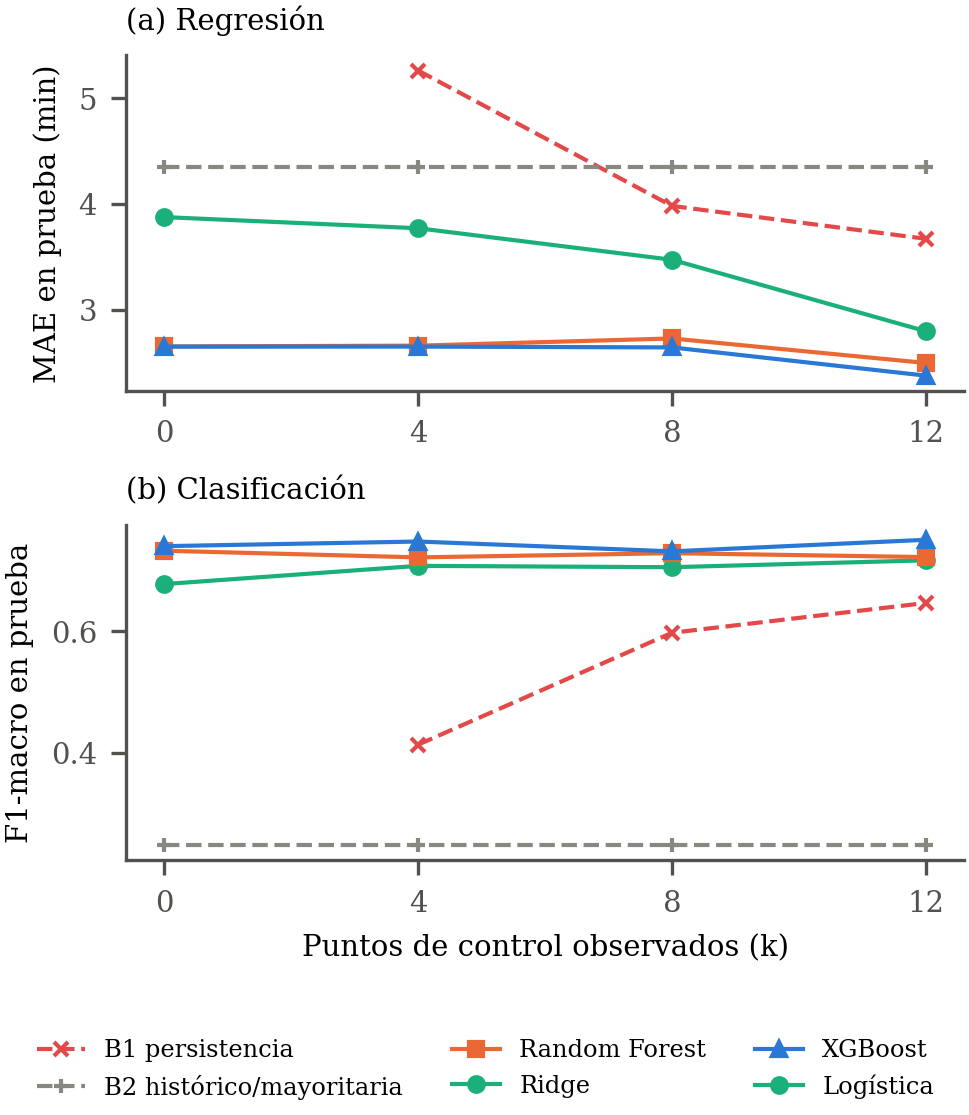
\includegraphics[width=\columnwidth]{fig/paper_fig5_efecto_k.png}
\caption{MAE (a) y F1-macro (b) en el conjunto de prueba según el número de PC observados (F0 en $k = 0$; F1 en $k > 0$). Líneas discontinuas: líneas base.}\label{fig:efectok}
\end{figure}

\begin{table}[!t]
\centering
\caption{$p$-valores del cambio entre escenarios consecutivos}\label{tab:h2}
\tabla{t_h2}

\vspace{2pt}\raggedright\scriptsize Wilcoxon sobre errores absolutos (regresión) y McNemar sobre aciertos (clasificación); F0 en $k = 0$ y F1 en $k > 0$. En negrita, $p < 0{,}05$. Los MAE correspondientes están en la Tabla~\ref{tab:testmae}.
\end{table}

\subsection{H3: aporte de las variables GPS}
Agregar los seis agregados GPS no mejora significativamente ningún modelo en ningún escenario (Tabla~\ref{tab:h3}). En validación cruzada, las diferencias entre F1 y F2 tampoco superan 0,03~min de MAE ni 0,011 de F1-macro, y ninguna variable GPS supera 0,02~min de importancia por permutación.

\begin{table}[!t]
\centering
\caption{Conjunto F1 frente a F2 en prueba}\label{tab:h3}
\tabla{t_h3}
\end{table}

\subsection{XGBoost frente a Random Forest}\label{sec:res-rf}
Ambos ensambles quedan cerca en todos los escenarios (Tabla~\ref{tab:xgbrf}). Con la corrección de Holm, XGBoost solo es significativamente mejor en regresión con $k = 12$ (2,37 frente a 2,49~min con F1, y 2,35 frente a 2,55 con F2) y en clasificación con $k = 4$ y $k = 12$ (F1). Antes de la salida son equivalentes: la ventaja de XGBoost aparece cuando el modelo debe combinar el contexto del itinerario con la información en ruta.

\begin{table}[!t]
\centering
\caption{XGBoost frente a Random Forest en prueba}\label{tab:xgbrf}
\tabla{t_xgb_rf}

\vspace{2pt}\raggedright\scriptsize Wilcoxon (MAE) y McNemar (F1-macro), con corrección de Holm por 7 escenarios. En negrita, $p_{\text{Holm}} < 0{,}05$.
\end{table}

\subsection{Detalle de la clasificación}
Las confusiones ocurren solo entre clases vecinas: ninguna vuelta retrasada se clasifica como adelantada ni viceversa antes de la salida (Fig.~\ref{fig:conf}). La Tabla~\ref{tab:sens} detalla la sensibilidad y la especificidad de cada clase. Antes de la salida, XGBoost alcanza una exactitud de 0,780 (0,592 la clase mayoritaria), una exactitud balanceada de 0,722 y un kappa de 0,595. ``Puntual'' se reconoce bien (sensibilidad 0,86) y las especificidades de ``adelantado'' y ``retrasado'' son altas (0,97 y 0,92): cuando el modelo anuncia un adelanto o un retraso, casi siempre ocurre. La clase más difícil es ``adelantado'': su sensibilidad es 0,54, porque casi la mitad de esas vueltas se predicen como puntuales. Con $k = 12$ mejora la detección de retrasos (sensibilidad de 0,77 a 0,83) a costa de más falsas alarmas (de 45 a 50 vueltas puntuales clasificadas como retrasadas).

\textbf{Pesos por clase.} La regla de decisión ponderada solo pasa la regla de aceptación en $k = 12$ con F1 (pesos 1,7 para ``adelantado'' y 1,0 para ``retrasado''; F1-macro de validación 0,734 $\rightarrow$ 0,736, 3 de 4 pliegues); en los otros seis escenarios empeora la validación y se descarta. En prueba, con $k = 12$, sube la sensibilidad de ``adelantado'' de 0,53 a 0,59 y el F1-macro de 0,751 a 0,759, pero la diferencia no es significativa (McNemar $p = 1{,}0$).

\begin{figure}[!t]
\centering
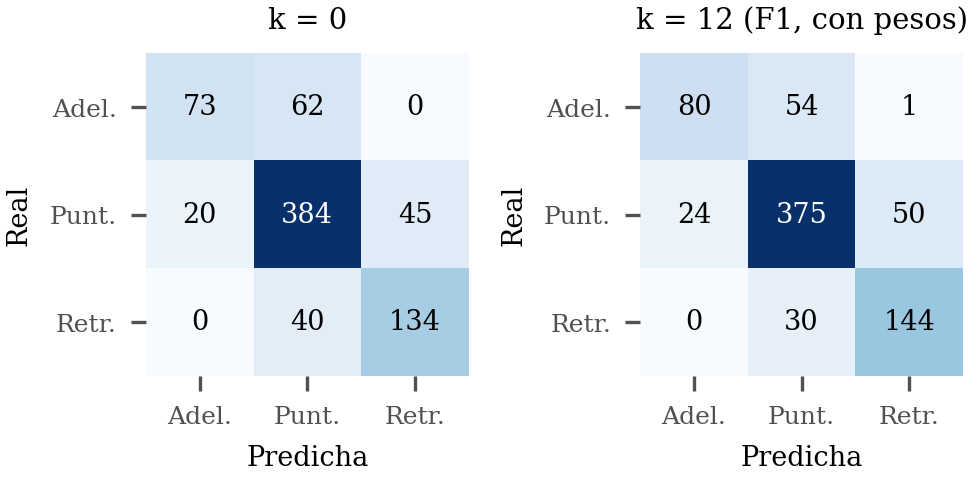
\includegraphics[width=\columnwidth]{fig/paper_fig6_confusion.png}
\caption{Matrices de confusión de XGBoost en el conjunto de prueba antes de la salida ($k = 0$) y con 12 PC observados (F1, con pesos por clase).}\label{fig:conf}
\end{figure}

\begin{table*}[!t]
\centering
\caption{Exactitud, exactitud balanceada, kappa y sensibilidad / especificidad por clase en prueba}\label{tab:sens}
\tablesize\setlength{\tabcolsep}{2.5pt}
\begin{tabular}{@{}lcccccc@{}}
\toprule
 & & & & \multicolumn{3}{c}{Sensibilidad / especificidad} \\
\cmidrule(l){5-7}
Modelo & Exact. & Exact. bal. & $\kappa$ & Adelantado & Puntual & Retrasado \\
\midrule
XGB, $k=0$ & 0,780 & 0,722 & 0,595 & 0,54 / 0,97 & 0,86 / 0,67 & 0,77 / 0,92 \\
XGB, $k=12$ F1 & 0,790 & 0,736 & 0,617 & 0,53 / 0,98 & 0,86 / 0,70 & 0,83 / 0,91 \\
XGB, $k=12$ F1 + pesos & 0,790 & 0,752 & 0,624 & 0,59 / 0,96 & 0,84 / 0,73 & 0,83 / 0,91 \\
Clase mayoritaria & 0,592 & 0,333 & 0,000 & 0,00 / 1,00 & 1,00 / 0,00 & 0,00 / 1,00 \\
\bottomrule
\end{tabular}


\vspace{2pt}\scriptsize Umbrales $-1/+5$~min. Sensibilidad y especificidad de cada clase frente al resto. La clase mayoritaria predice siempre ``puntual''.
\end{table*}

\subsection{Análisis de sensibilidad de los umbrales de clase}\label{sec:res-umbrales}
Con la tolerancia amplia ($-3/+10$~min), la exactitud de XGBoost sube a 0,832 con $k = 0$ y a 0,871 con $k = 12$ (Tabla~\ref{tab:umbrales}), pero la de la clase mayoritaria sube aún más, de 0,592 a 0,788, porque ``puntual'' pasa a ser el 78\,\% de las vueltas. El kappa, que descuenta ese acierto por azar, apenas cambia antes de la salida (0,595 frente a 0,601). Es decir, la mayor exactitud con umbrales tolerantes se debe sobre todo a que el problema es más fácil, no a un mejor modelo; por eso se mantiene la definición $-1/+5$.

\begin{table}[!t]
\centering
\caption{Clasificación con umbrales principales y con tolerancia amplia (XGBoost, prueba)}\label{tab:umbrales}
\tabla{t_umbrales}

\vspace{2pt}\raggedright\scriptsize Exact. mayor.: exactitud de la clase mayoritaria con esos umbrales.
\end{table}

\subsection{Error por día en el conjunto de prueba}
El sábado concentra el error: el MAE de XGBoost antes de la salida es 5,40~min ese día, frente a 1,88--2,74~min de martes a viernes (Tabla~\ref{tab:dia}). El sábado es el 14\,\% de las vueltas de prueba, pero aporta el 28\,\% del error absoluto total.

\begin{table}[!t]
\centering
\caption{Error de XGBoost ($k = 0$) por día de prueba}\label{tab:dia}
\tabla{t_dia}
\end{table}

\subsection{Variables del día en curso}
Ninguno de los grupos de variables del día pasa la regla de aceptación (Tabla~\ref{tab:cribado}). C, P y C+P empeoran el MAE de validación entre 0,02 y 0,06~min y el F1-macro entre 0,008 y 0,022. El diagnóstico de C es que el retraso medio de las vueltas ya terminadas está confundido con la hora: antes de las 8~h solo han terminado vueltas de madrugada, que van adelantadas. La anomalía del día (A), que corrige ese sesgo, solo mejora en regresión con $k = 12$ ($-$0,04~min, 3 de 4 pliegues) y empeora en los otros tres casos; como la mejora no es consistente y está en el orden de la variación entre plataformas, tampoco se adopta.

\begin{table}[!t]
\centering
\caption{Cribado de variables del día en curso (validación, XGBoost)}\label{tab:cribado}
\tabla{t_cribado}

\vspace{2pt}\raggedright\scriptsize Media de validación; entre paréntesis, pliegues en que mejora a la base. Regla de aceptación: mejor media y al menos 3 de 4 pliegues.
\end{table}

\subsection{Importancia de las variables y explicaciones SHAP}
La hora programada de salida es la variable más importante en todos los casos (Fig.~\ref{fig:imp}). En el modelo de regresión antes de la salida, permutarla aumenta el MAE en 3,97~min; el día de la semana lo aumenta en 1,60~min, y el horario, el vehículo y el número de vuelta, en menos de 0,25~min cada uno. Con $k = 12$ y GPS, la hora conserva el primer lugar (2,27~min) y la desviación en PC12 pasa al segundo (1,26~min), seguidas del día (0,42~min).

\begin{figure}[!t]
\centering
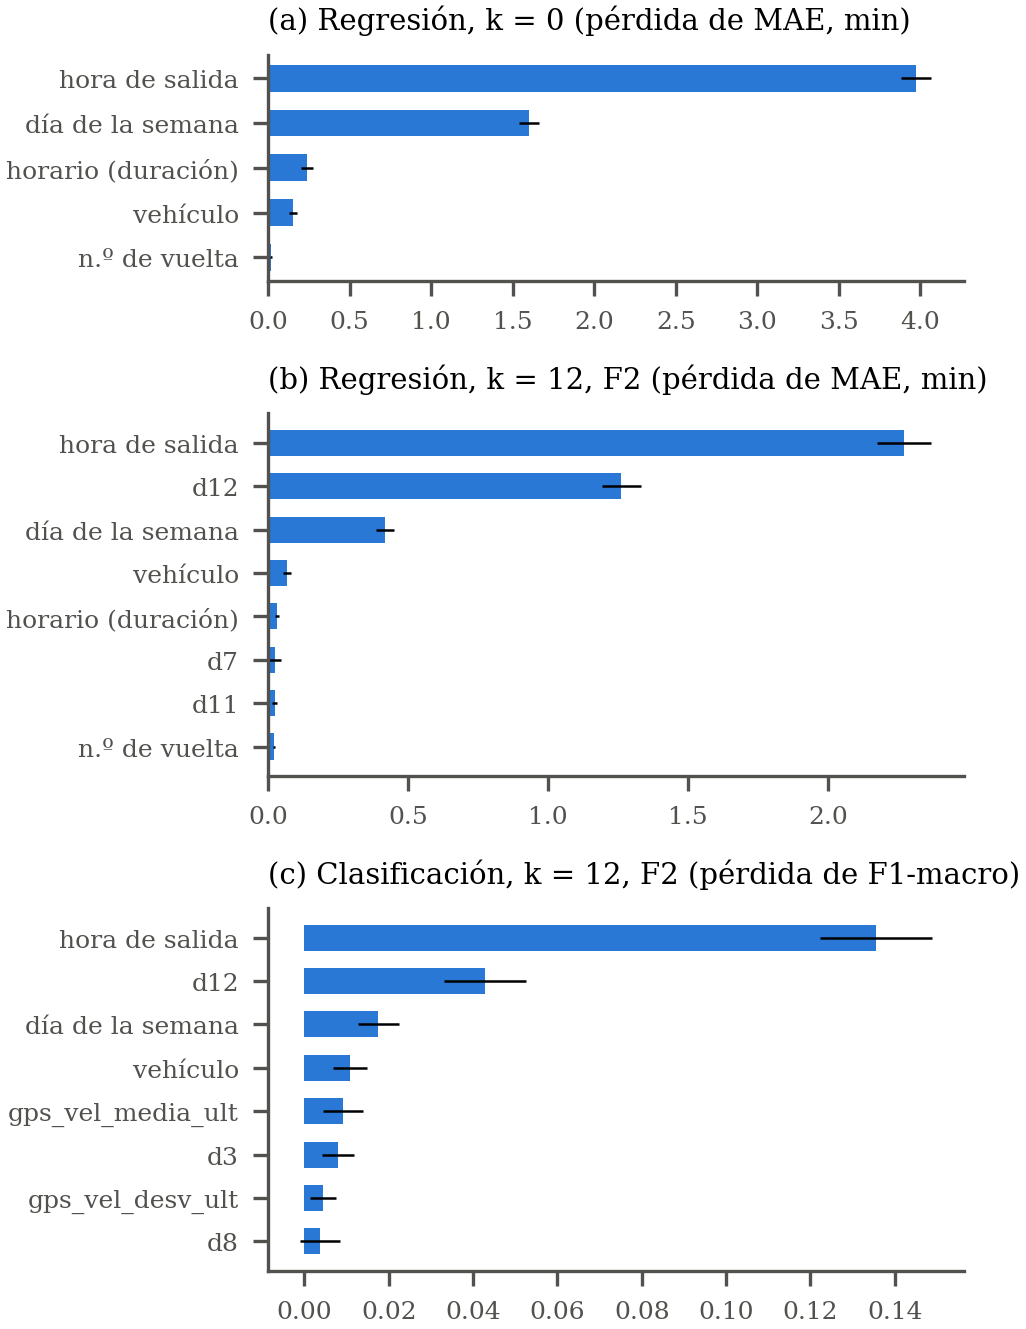
\includegraphics[width=\columnwidth]{fig/paper_fig7_importancia.png}
\caption{Importancia por permutación en prueba (10 repeticiones; barras: desviación estándar) de los mejores modelos (XGBoost): (a) regresión con $k = 0$, (b) regresión con $k = 12$ y F2, (c) clasificación con $k = 12$ y F2.}\label{fig:imp}
\end{figure}

Los valores SHAP muestran \emph{cómo} actúan esas variables (Fig.~\ref{fig:shap}). La hora de salida desplaza la predicción desde unos $-25$~min en las salidas de madrugada hasta +12~min en las de la tarde, y el día de la semana separa dos grupos: los días laborables restan alrededor de 2~min y el sábado suma entre 5 y 10~min. La Fig.~\ref{fig:shapsab} explica una vuelta concreta del sábado 01/02 con salida a las 17:54: partiendo del promedio de 2,8~min, la hora suma 12,2~min, el sábado 9,0~min, el horario 1,1~min y el vehículo 0,7~min, para una predicción de 26,0~min frente a 29~min reales.

\begin{figure}[!t]
\centering
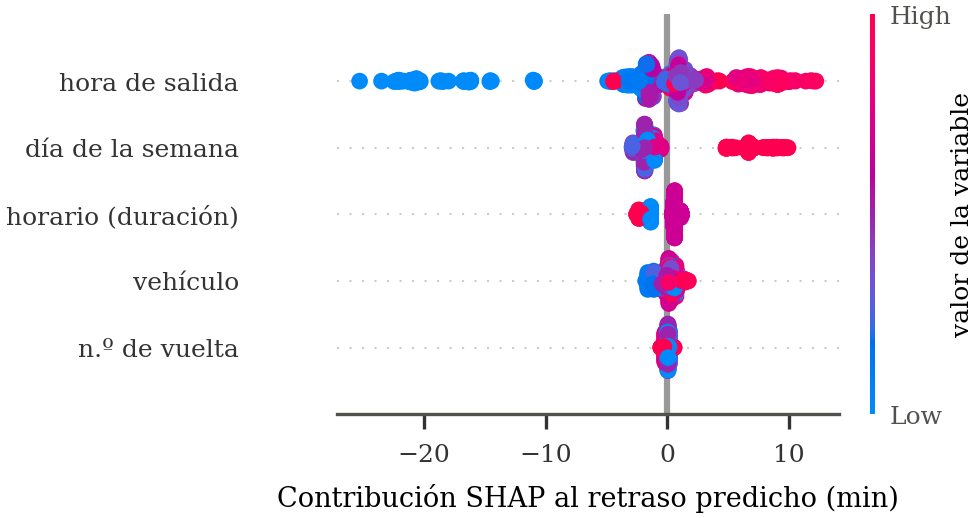
\includegraphics[width=\columnwidth]{fig/paper_fig8_shap.png}
\caption{Valores SHAP de XGBoost (regresión, $k = 0$) en las 758 vueltas de prueba. Cada punto es una vuelta; el color indica el valor de la variable (rojo: alto; azul: bajo). Día de la semana: 0 = lunes, \ldots, 5 = sábado.}\label{fig:shap}
\end{figure}

\begin{figure}[!t]
\centering
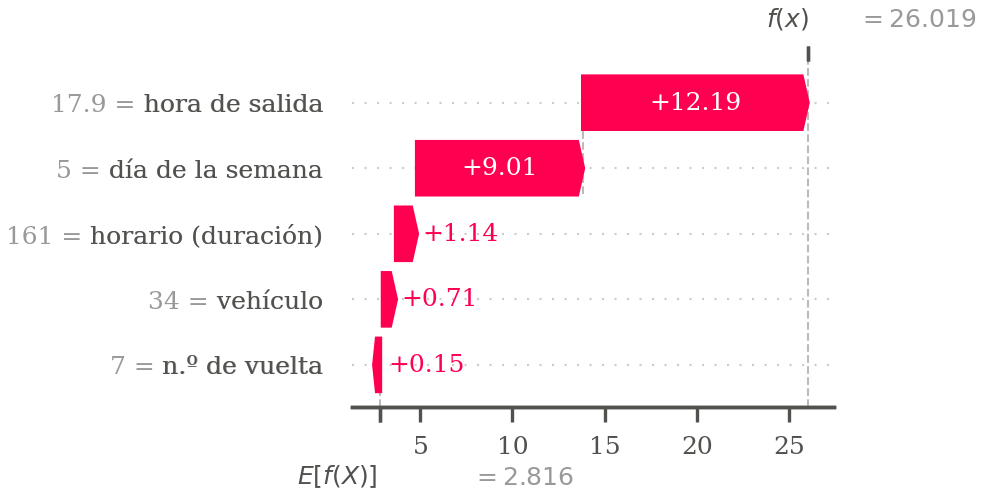
\includegraphics[width=\columnwidth]{fig/paper_fig9_shap_sabado.png}
\caption{Explicación SHAP de la predicción de una vuelta del sábado 01/02 con salida programada a las 17:54. $E[f(X)]$: predicción media del entrenamiento; $f(x)$: predicción de la vuelta.}\label{fig:shapsab}
\end{figure}

% =====================================================================================
\section{Discusión}\label{sec:disc}

\textbf{H1 se confirma.} Los tres modelos superan a las dos líneas base, y el mejor lo hace con amplio margen y significancia en todos los escenarios. Que el promedio histórico por hora explique el 43\,\% de la varianza ($R^2 = 0{,}43$) y XGBoost el 75\,\% sin información en ruta indica que el retraso responde a regularidades que una regla de una sola variable no captura: la interacción entre hora, día de la semana y horario programado. Que XGBoost elija árboles de profundidad 2 antes de la salida refuerza esta lectura: bastan interacciones de dos variables, como hora $\times$ día. La persistencia es la peor referencia al inicio de la vuelta ($R^2 \approx 0$ con $k = 4$): un adelanto o retraso temprano no se arrastra hasta el final.

\textbf{H2 se confirma solo en parte.} El error no baja de forma monótona con $k$. En los modelos de árboles, conocer los primeros 4 u 8 PC no aporta, y la mejora aparece recién con $k = 12$ ($-$10\,\% de MAE con XGBoost). Esto coincide con el análisis exploratorio: la desviación en PC1--PC3 no está correlacionada con la final, y los tramos que más retraso generan o recuperan (PC13--PC14, junto al mercado San Pedro, y PC14--PC15) están en la segunda mitad. Para la gestión de la flota, la predicción antes de la salida es casi tan buena como la de mitad de recorrido, y la actualización en ruta vale la pena a partir del retorno desde el centro. Es también en ese momento cuando XGBoost supera de forma significativa a Random Forest.

\textbf{H3 se rechaza en esta formulación.} Seis agregados GPS, calculados sin fuga y con el tiempo detenido medido como duración, no mejoran el error en ningún modelo ni escenario, y su importancia por permutación es casi nula. Una explicación plausible es que la desviación en los PC ya resume lo que el GPS mide: si el bus estuvo detenido o lento, ya llegó tarde al PC. El resultado contrasta con Meyer-Hollatz et~al.~\cite{meyer2023}, donde agregar clima y feriados redujo el MAE en 17\,\%; esas variables son externas al registro de operación y aportan información nueva, mientras que los agregados GPS son redundantes con los PC. Es un resultado nulo bien medido, con pruebas pareadas y en tres familias de modelos.

\textbf{Resultados negativos de las mejoras.} Ni las variables del día en curso ni la regla de decisión ponderada mejoran de forma consistente, pese a que el sábado concentra el 28\,\% del error. Con 10 a 19 días de entrenamiento por pliegue, el modelo ve muy pocos ``estados del día'' distintos (tres sábados en el desarrollo) para aprender cómo un mal inicio de jornada anticipa el resto. Haber fijado la regla de aceptación antes de los experimentos permite reportar estos resultados como hallazgos y no como intentos descartados.

\textbf{El retraso es mayormente sistemático.} La hora de salida y el día de la semana dominan la importancia por permutación y las explicaciones SHAP, y el sábado agrega en promedio entre 8 y 10~min de retraso respecto de los días laborables. Esto es coherente con la observación de campo: el retraso crece cuando hay más pasajeros y los buses esperan para llenarse, y en la madrugada los buses adelantan. Que el horario de 170~min, que asigna más tiempo, tenga el peor cumplimiento (53,7\,\% con más de 5~min de retraso) sugiere que los tiempos programados no reflejan la demanda real de la tarde. Si el retraso es predecible desde el itinerario, recalibrar los horarios por franja y día puede reducirlo tanto como el control en tiempo real.

\textbf{Comparación con la literatura.} El MAE de 2,4--2,7~min es menor que los $\sim$3,6~min de Martyanov et~al.~\cite{martyanov2026} con modelos similares, aunque las tareas difieren: ellos predicen el retraso en cada parada y aquí solo el final de la vuelta, con una ruta y un mes. Como en~\cite{martyanov2026} y~\cite{taparia2020}, los ensambles de árboles superan a los modelos lineales, y como en~\cite{meyer2023}, XGBoost es el mejor modelo. La clasificación en tres clases de Cao et~al.~\cite{cao2017} se replicó con un F1-macro de 0,73--0,76, una exactitud de 0,77--0,79 y un recall de ``retrasado'' de hasta 0,88, la clase de mayor interés para el operador~\cite{sun2021}.

\textbf{Elección del modelo.} XGBoost es la mejor opción general, pero antes de la salida Random Forest es equivalente. Si el operador prioriza no dejar pasar retrasos, Random Forest con ponderación balanceada detecta más vueltas retrasadas (0,86--0,88) con un F1-macro apenas menor.

% =====================================================================================
\section{Limitaciones y amenazas a la validez}\label{sec:lim}

El dataset cubre 27 días de una sola ruta, por lo que no permite evaluar estacionalidad, temporada de lluvias, feriados ni generalización a otras rutas. El conjunto de prueba es pequeño y abarca de martes a sábado: incluye un solo sábado y ningún domingo ni lunes. El sábado concentra el mayor error (Tabla~\ref{tab:dia}), de modo que el desempeño en ese día descansa en una sola jornada de 105 vueltas; para domingo y lunes solo se dispone de la estimación de la validación cruzada, cuyos pliegues 2 y 4 sí los contienen.

El MAE de prueba (2,65~min con XGBoost en $k = 0$) es menor que el de validación (3,12 $\pm$ 0,88~min) en todos los modelos. La variabilidad entre pliegues es alta y la prueba tiene cuatro días laborables con poco retraso, por lo que las cifras de prueba deben leerse junto con la media y la desviación de la validación.

Los resultados de XGBoost con submuestreo dependen levemente de la plataforma y del número de hilos; las cifras finales son deterministas en la máquina en que se obtuvieron, pero pueden variar unas centésimas en otra. Las conclusiones no dependen de esas diferencias, que son menores que la variación entre pliegues. Los óptimos de XGBoost en $k = 12$ (1\,600 árboles, tasa 0,01) quedaron otra vez en el borde de la malla, por lo que aún podría ganarse algo con más árboles.

La desviación está truncada a minutos, lo que limita la resolución del objetivo y de los umbrales de clase. La semántica de \texttt{Times.csv} se infirió numéricamente, difiere del README y está pendiente de confirmación por los docentes. Al ser datos observacionales sin conteo de pasajeros, el estudio identifica asociaciones (por ejemplo, entre el sábado y el retraso) pero no causas; los valores SHAP explican el modelo, no el mecanismo del retraso.

% =====================================================================================
\section{Conclusiones y trabajo futuro}\label{sec:conc}

Es posible anticipar con buena precisión el retraso con que un bus de esta ruta terminará su vuelta, incluso antes de que salga: XGBoost logra un MAE de 2,65~min, un F1-macro de 0,740 y una exactitud de 0,78 solo con el contexto del itinerario, un 39\,\% menos de error que el promedio histórico. La información en ruta mejora la predicción de forma significativa solo a partir del PC12, y es entonces cuando XGBoost supera a Random Forest; los agregados GPS y las variables del día en curso no aportan. La hora de salida y el día de la semana, con el sábado como caso extremo, explican la mayor parte del retraso, como muestran tanto la importancia por permutación como los valores SHAP. Para el operador, la implicancia principal es que recalibrar el itinerario por franja horaria y día, en particular las tardes y los sábados, ataca la causa sistemática del retraso.

Como trabajo futuro se propone: (i) ampliar el periodo de datos para cubrir varios meses, más sábados y la temporada de lluvias, lo que permitiría que las variables del estado del día aporten; (ii) incorporar variables externas al registro de operación, como clima, feriados y eventos, que en~\cite{meyer2023} sí mejoraron la predicción; (iii) predecir el retraso en cada PC y no solo al final de la vuelta, y (iv) evaluar la recalibración del itinerario propuesta simulando horarios ajustados con el modelo.
% TODO (demo): cuando la demostración interactiva esté lista, agregar aquí una oración que la describa
% (mapa de la ruta con los 18 PC y selectores de hora, día y n.º de PC observados).

% =====================================================================================
\begin{thebibliography}{99}
\bibitem{alexandre2023} T.~Alexandre, F.~Bernardini, J.~Viterbo y C.~E.~Pantoja, ``Machine learning applied to public transportation by bus: A systematic literature review,'' \emph{Transp. Res. Rec.}, vol.~2677, no.~7, pp.~639--660, 2023.
\bibitem{singh2022} N.~Singh y K.~Kumar, ``A review of bus arrival time prediction using artificial intelligence,'' \emph{WIREs Data Mining Knowl. Discov.}, vol.~12, no.~4, e1457, 2022, doi: 10.1002/widm.1457.
\bibitem{lin1999} W.-H.~Lin y J.~Zeng, ``Experimental study of real-time bus arrival time prediction with GPS data,'' \emph{Transp. Res. Rec.}, no.~1666, pp.~101--109, 1999.
\bibitem{rashvand2024} N.~Rashvand, S.~S.~Hosseini, M.~Azarbayjani y H.~Tabkhi, ``Real-time bus arrival prediction: A deep learning approach for enhanced urban mobility,'' SciTePress, 2024, pp.~123--132, doi: 10.5220/0012365500003639.
\bibitem{jeong2005} R.~Jeong y L.~R.~Rilett, ``Prediction model of bus arrival time for real-time applications,'' \emph{Transp. Res. Rec.}, vol.~1927, no.~1, pp.~195--204, 2005, doi: 10.1177/0361198105192700123.
\bibitem{liu2020} D.~Liu, J.~Sun y S.~Wang, ``BusTime: Which is the right prediction model for my bus arrival time?,'' arXiv:2003.10373, 2020.
\bibitem{martyanov2026} V.~Martyanov, A.~Budzyński, A.~Czerepicki y M.~Kozłowski, ``Interpretable machine learning for identifying the determinants of bus delays,'' \emph{Archives of Transport}, vol.~77, no.~1, pp.~7--26, 2026, doi: 10.61089/aot2026.mnrkh112.
\bibitem{meyer2023} T.~Meyer-Hollatz, N.~Schwarz y T.~Werner, ``Punctuality predictions in public transportation: Quantifying the effect of external factors,'' en \emph{Proc. Wirtschaftsinformatik 2023}, art.~73, 2023.
\bibitem{taparia2020} A.~Taparia, ``Bus journey and arrival time prediction based on archived AVL/GPS data using machine learning,'' tesis de maestría, Trinity College Dublin, Dublín, Irlanda, 2020.
\bibitem{cao2017} H.~Cao, M.~Wachowicz, C.~Renso y E.~Carlini, ``An edge-fog-cloud platform for anticipatory learning process designed for Internet of Mobile Things,'' arXiv:1711.09745, 2017.
\bibitem{sun2021} W.~Sun, J.-D.~Schmöcker y T.~Nakamura, ``On the trade-off between sensitivity and specificity in bus bunching prediction,'' \emph{J. Intell. Transp. Syst.}, vol.~25, no.~4, pp.~384--400, 2021, doi: 10.1080/15472450.2020.1725887.
\bibitem{yu2016} H.~Yu, D.~Chen, Z.~Wu, X.~Ma y Y.~Wang, ``Headway-based bus bunching prediction using transit smart card data,'' \emph{Transp. Res. Part C Emerg. Technol.}, vol.~72, pp.~45--59, 2016, doi: 10.1016/j.trc.2016.09.007.
\bibitem{hoerl1970} A.~E.~Hoerl y R.~W.~Kennard, ``Ridge regression: Biased estimation for nonorthogonal problems,'' \emph{Technometrics}, vol.~12, no.~1, pp.~55--67, 1970.
\bibitem{hastie2009} T.~Hastie, R.~Tibshirani y J.~Friedman, \emph{The Elements of Statistical Learning}, 2.ª~ed. Nueva York, NY, EE.\,UU.: Springer, 2009.
\bibitem{breiman2001} L.~Breiman, ``Random forests,'' \emph{Mach. Learn.}, vol.~45, no.~1, pp.~5--32, 2001.
\bibitem{friedman2001} J.~H.~Friedman, ``Greedy function approximation: A gradient boosting machine,'' \emph{Ann. Statist.}, vol.~29, no.~5, pp.~1189--1232, 2001.
\bibitem{chen2016} T.~Chen y C.~Guestrin, ``XGBoost: A scalable tree boosting system,'' en \emph{Proc. 22nd ACM SIGKDD Int. Conf. Knowl. Discov. Data Mining}, 2016, pp.~785--794, doi: 10.1145/2939672.2939785.
\bibitem{pedregosa2011} F.~Pedregosa et~al., ``Scikit-learn: Machine learning in Python,'' \emph{J. Mach. Learn. Res.}, vol.~12, pp.~2825--2830, 2011.
\bibitem{wilcoxon1945} F.~Wilcoxon, ``Individual comparisons by ranking methods,'' \emph{Biometrics Bull.}, vol.~1, no.~6, pp.~80--83, 1945.
\bibitem{mcnemar1947} Q.~McNemar, ``Note on the sampling error of the difference between correlated proportions or percentages,'' \emph{Psychometrika}, vol.~12, no.~2, pp.~153--157, 1947.
% TODO: verificar la página o capítulo exacto del TCQSM donde aparece la definición de puntualidad "1 min antes – 5 min después".
\bibitem{tcqsm2013} Kittelson \& Associates et~al., \emph{Transit Capacity and Quality of Service Manual}, 3.ª~ed., TCRP Report 165. Washington, DC, EE.\,UU.: Transportation Research Board, 2013.
\bibitem{cohen1960} J.~Cohen, ``A coefficient of agreement for nominal scales,'' \emph{Educ. Psychol. Meas.}, vol.~20, no.~1, pp.~37--46, 1960.
\bibitem{holm1979} S.~Holm, ``A simple sequentially rejective multiple test procedure,'' \emph{Scand. J. Statist.}, vol.~6, no.~2, pp.~65--70, 1979.
\bibitem{lundberg2017} S.~M.~Lundberg y S.-I.~Lee, ``A unified approach to interpreting model predictions,'' en \emph{Advances in Neural Information Processing Systems 30}, 2017, pp.~4765--4774.
\end{thebibliography}

\end{document}
